\section{Protocol communication}\label{cha:protocolDesign}
\todo{be more humble, analytic and include possibilities or explain why omitted}
To transmit the data from the nodes to the main node, a protocol must be implemented.
The protocol must support the utilized hardware components and be designed to work within their limitations. 

The protocol to be developed for the solution will be based on the examination of networks in section \ref{fig:topologies} and the protocols described in section \ref{cha:comprot}.
There are a number of considerations to be made to develop a protocol that complies to the requirements.
Because the sensor nodes are battery driven, most of the choices are done with power consumption as a priority, to increase the battery longevity.

While the individual nodes have a relatively short communication range, a network of these devices can have a longer reach if the nodes are able to relay data through each other.
Therefore, relaying must be supported by the protocol as stated in \ref{cha:requirements}. 

For power consumption and complying to the usage, the network nodes are controlled by the main node, and the nodes will transmit sensor data on demand.
This implementation will keep the nodes in a low power listening mode until a data request is received.
The nodes transmitting their sensor readings automatically requires some sort of synchronization, so the node data is updated for every node and transmitted back to the main node.
There is no requirement for real-time monitoring of the golf course, making it difficult defining a data transfer interval that matches both power consumption as well as the need for information.
Hence, an on demand request for data will be sufficient.

\subsection{Transfer method and topology}
The solution must gather sensor data from all nodes in the network, and this subsection will contain the considerations made for the choice of topology.

To fulfill the requirements found in \ref{cha:requirements}, there is no demand to request data for only one specific node at a time.
There are multiple methods to request data from the network nodes, some of the most used ones can be found in \ref{cha:comprot}. 
\iffalse
One way of requesting data can be done by transmitting a data request to every node in the network, addressing the nodes by name. This would require the main node to create an individual request to each node in the network, and the network nodes to know the path through the network to the addressee, so that the request can be relayed correctly. This is not appropriate when the network nodes have limited memory\todo{how much would routing tables fill?}. In case of disconnected nodes, the routing tables must be reconfigured, to make sure packets are relayed in a path that does exist. This would accordingly require nodes to somehow broadcast that they are still alive, and thereby consume more energy.
\fi

The protocol selected for the solution is partly based on the flooding protocol.
This protocol is a method where the data request can be transmitted by flooding the network, without needing to send a tailored request to every node in the network. 
A data request will be broadcasted to all nodes in the network, using flooding, and will only require one packet. 
If the broadcast is done by controlled flooding, there will be no cycles, and the outgoing transmit topology will consequently be a tree. 
Flooding will only handle one packet, but the nodes can receive the same packet multiple times and must analyze and discard any duplicate packets.

The controlled flooding has a low memory impact and thus best suited for the solution. The flooding protocol will create a tree which can be utilized to create a return path for the nodes' sensor readings.

\begin{figure}[h!]
	\centering
	\makebox[\textwidth][c]{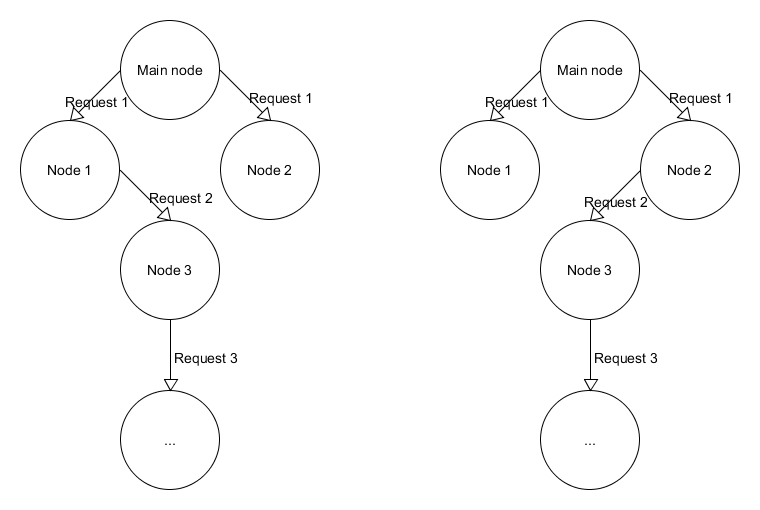
\includegraphics[scale=0.4]{chapters/design/figures/branchExample.png}}
	\caption{The trees structure can vary depending on the node that connects to the main node first.}
	\label{fig:treeVariation}
\end{figure}

The tree created in each request broadcast can vary in its structure, depending on interference, removal of nodes or faulty nodes or by other occurrences. \figref{treeVariation} shows an example of how the tree can vary: first the main node will broadcast "request 1", which is received by both "node 1" and "node 2". An external node in the system will always handle its own sensor data before it starts relaying data from other nodes. If the main node receives data from "node 1" first, then the resulting tree will match the tree seen to the left if \figref{treeVariation}. If "node 2" connects to the main node first, then the tree will match the tree on the right.
This will effectively solve the requirement of respond appropriately to a disconnecting node as well as including new nodes in the network, since a new tree is constructed with each wave of requests from the main node.
It will also use the shortest paths to every node, due to each node connecting to its immediate neighbors.

The tree instantiated by the flood, can be used to create a path from each node to the main node.
The receiver of a request signal can use the sender as the parent when data is to be returned.
The child will then repeat the request signal, and be the parent of nodes hearing it.

The topology of the network will effectively be a tree, although prone to changes in branches.
Any node receiving a request signal will then be able to respond to its parent, causing all nodes to have a single identifier for the routing towards the destination node, the main node.

\subsection{Sequence}
The protocol sequence is determined as the following. A flowchart can be seen in the appendix.\todo{add flowchart to appendix}

This is the operation structure for each individual node in the system.
\begin{enumerate}
	\item Receive data request (Wireless request for nodes, user input at the main node)
	\subitem Ignore if (already received or not recipient of package)
	\item Remember parent (MN skip)
	\item Acquire sensor data
	\item Send sensor data to parent (if silence?)
	\item Receive acknowledgment of sent package
	\item Send data request to all
	\item Receive data from children
	\item If no response or acknowledgment within 10 min: (deep) sleep?
\end{enumerate}

\subsection{Interference handling} \label{cha:crcDesign}
When utilizing wireless communication, interference can be a problem, as explained in section \ref{cha:floodingSec}. This is also the case when using controlled flooding, but using a protocol can help reduce problems with interference, for instance by validating the transferred data and acting accordingly.

Interference might scramble packets, which makes it impossible to use the received data. Figure \ref{fig:prottree1} shows an example of a possible interference scenario, where nodes 5, 6, and 7 could send packets at the same time, causing node 3 to receive scrambled data.

To ensure this is not a problem, a checksum is used for verifying packets. This checksum is transmitted with the data and recipient. When a node receives a packet, this checksum is calculated, and compared to the one in the packet. If the checksums match, the packet is accepted and can be relayed to the next node. This will cause the receiving node to send an acknowledgment to the node that sent the packet, which will then stop transmitting data.
If the checksums do not match, the packet is ignored until a packet that have the same checksum makes its way to the node. \todo{move to checksum/data verification}

To ensure that a packet with the correct checksum will arrive at some point, the nodes will wait a random, but longer, interval between attempting to send data. This means that at some point, the data will be transmitted to the receiver without interference.
This is possible, as time is not essential, and the delay between trying again is short.


\subsection*{Example}
The protocol uses flooding to distribute the data request through the network. 
When data is requested by the user, the main node sends a packet containing a sensor reading request. 
The nodes that receive this packet directly from the main node is the first level of nodes in the tree, as seen in figure \ref{fig:prottree1}. 
These nodes then read the moisture values from their sensors and transmit these back to the main node. 

The first level nodes then request data from the nodes within their range. 
The nodes receiving this request firstly verifies that it is a new request, then registers the node that requested data as its parent. 
These nodes are second level nodes. The second level nodes read from the sensors, and sends data back to their parents. The parents then relay the data to the main node. 
This procedure continues until all reachable sensors have relayed data back to the main node.
An illustration showing an example of a tree is seen on Figure \ref{fig:prottree1}.

For each new data request from the main node the tree structure and node levels are assessed again as they might have changed, due to new or disconnected nodes.

\begin{figure}[!h]
	\centering
	\makebox[\textwidth][c]{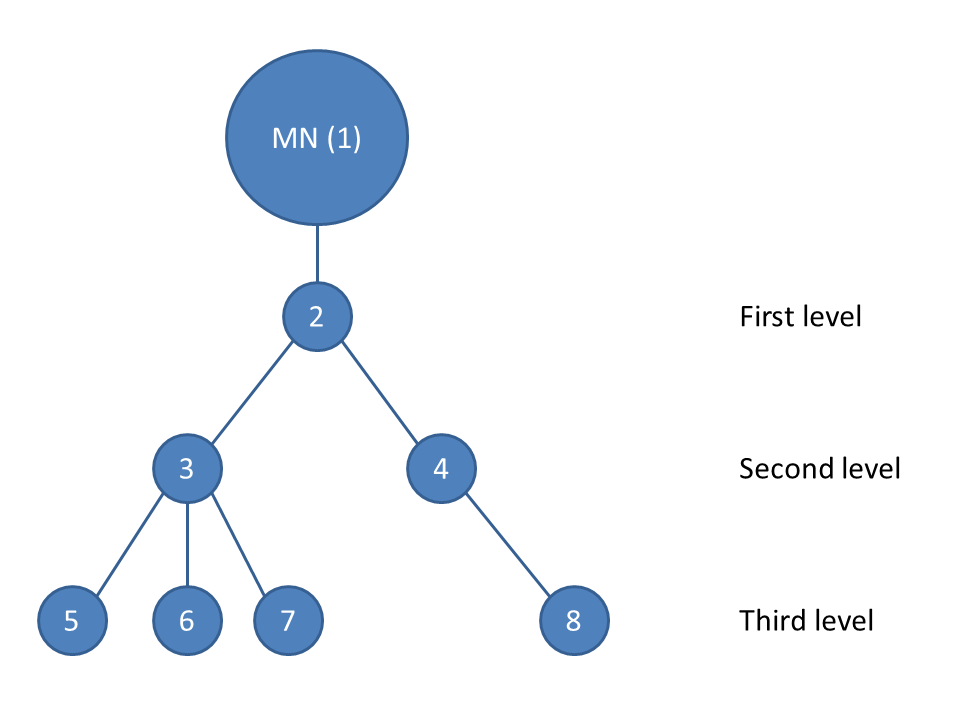
\includegraphics[width=1\textwidth]{chapters/design/figures/prottree1.png}}
	\caption{Example of a tree.}
	\label{fig:prottree1}
\end{figure}








\section{Protocol packet}
This section covers the descriptions and decisions regarding the packets in the system.


\subsubsection{Packet types}
There are multiple types of data needed to make a functioning protocol. The nRF24L01 supports data payloads up to 32 bytes, and is accordingly the limit of data to transfer in each packet.
Although, a decrease in amount of data can enable the protocol to be implemented on more limited hardware in addition to use less energy on broadcast.

There are five types of packages: pair request, data request, data response, acknowledgment and flush?
These are used to tell the receiver what kind of data the packet contains, so that the receiving node can decide how to handle the received packet. 1 byte will be sufficient to store the packet type.
The five packet types are described followingly.

\textit{Pair request}\newline
A pair request is a packet send from the main node, the raspberry pi.
The packet will be read by a single sensor node set to be paired with the network.
When the two nodes, main and sensor node, are paired, the sensor node knows what networks it belongs to, and can then be deployed in the field as a park of the network. 

\textit{Data request}\newline
A data request is a packet which the main node transmits to all sensor nodes within range.
Each sensor node then relay the data request out though the network.
The packet contains the ID of the previous node transmitting it, so each sensor node receiving the packet, knows where it comes from.

\textit{Data response}\newline
A data response is a response to the data request.
A sensor node which receive a data request will transmit a packet with data back to its parent.
The parent is whom the data request came from.

\textit{Acknowledgment}\newline
An acknowledgment packet is a packet which is expected to be received after a data response packet have been delivered.
The packet is only to make sure the recorded date from the sensor nodes reach another node, and is not lost.

\textit{Flush}\newline
Flush is used to reset every node in the network, this will happen when all data is collected.
The flush packet let every node in the network know that it should forget any previous information stored, such as parent information.

\subsubsection{Other data}
There has to be an addresser and an addressee.\todo{why?} These are the 'from' and 'to' parts of the packet, and specifies which node the packet is for, and which node the packet is sent from.
Since the data sent with the package not necessarily originates from the same node from which it is sent, because of relaying in the network, there also needs to be data allocated to identify the origin.
The limitation of the network size is 1000 nodes, the identifier data fields needs to support 1000 unique addresses, which requires 9 bits. The allocated size for the addresses are accordingly 2 bytes(16 bits) each to maintain usage of whole bytes. This is done because it is more efficient to manipulate a byte instead of a bit \cite{bytevsbit}. The addresses requires 6 bytes in total.

To verify the integrity of the received package, a Cyclic redundancy check (CRC16) is appended. CRC16 uses 2 bytes to distinguish a successfully transfered packet from an erroneous one. 

To support multiple sensors per node, there are three fields allocated for sensor data.
The readings of the moisture sensor have a resolution of 1024 values, and the required size allocated for the sensor reading data is 10 bits. The allocated data size in the transfer is therefore 2 bytes.

\begin{figure}[h!]
	\centering
	\makebox[\textwidth][c]{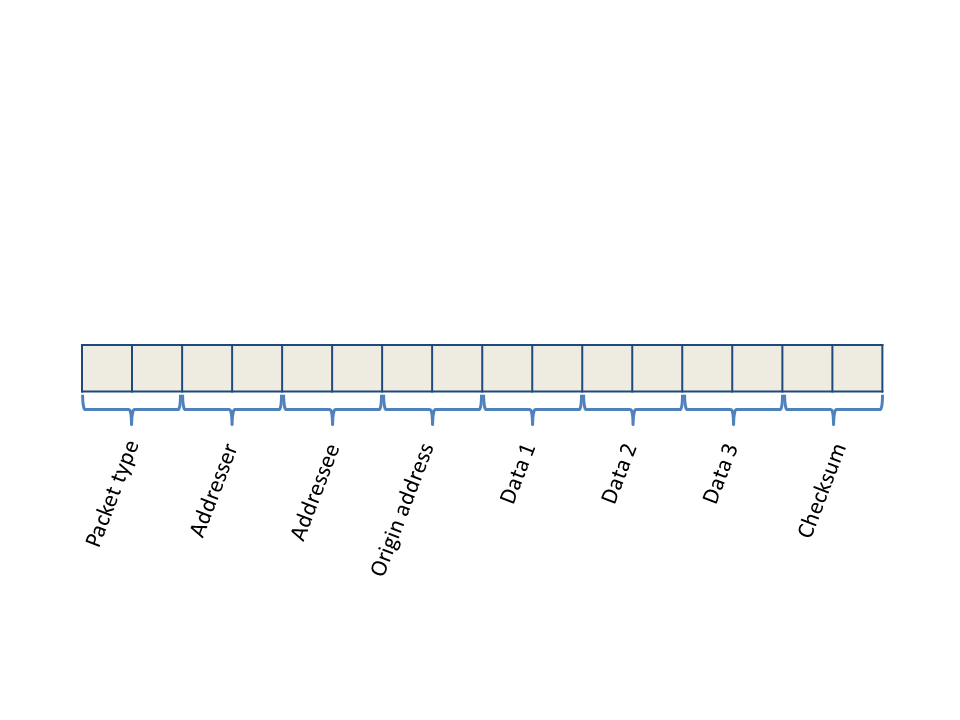
\includegraphics[width=1\textwidth,trim={0 3cm 0 8cm},clip]{figures/dataalloc.png}}
	\caption{Data allocation in packets.}
	\label{fig:dataalloc}
\end{figure}

The sizes of the different data to transfer sums up to 16 bytes and the distribution is displayed in \figref{dataalloc}.


\subsection{Packet data and allocation}
This section will contain elaborations regarding the data to be used in the protocol.\todo{explain "packet" somewhere earlier?}




\subsection{Verification of a message}
%Verification of a message
The received message is verified by doing one of the two following methods. 

Generate checksum of message m and compare with received checksum r.
The checksum of a correctly transferred packet $T$ is 0, because a package $T$, if correctly transferred, is some quotient $Q$ times the polynomial $G$, as seen in eqref[earlier]. If a division has a zero remainder, the packet was transferred correctly.




\subsection{Adding and removing nodes}
If a new node is to be added to the network, it needs an identifier in the system so that its sensor reading can be recognized. The identifier is permanent as long as it is in the network.
The identifier is provided by the main node by pairing the device with the main node before adding it to the network. 

The identifier is used to address parent nodes to relay the packets when transmitting sensor data. In figure \ref{fig:prottree1}, the nodes 5, 6, and 7 would send and address packets to the parent by the identifier 3. This means that other nodes in the vicinity would ignore these packets, and only node 3 reacts on the packets. Node 3 would then relay the data to node 2, as 2 is 3's parent, and finally 2 would relay to MN.

Should a node somehow disconnect from the network, the nodes connected to this node will receive the packets from another node first, and from that point on use that as the parent. This is if there are any nodes in range of the disconnected nodes' subnodes. 

\begin{figure}[!h]
	\centering
	\makebox[\textwidth][c]{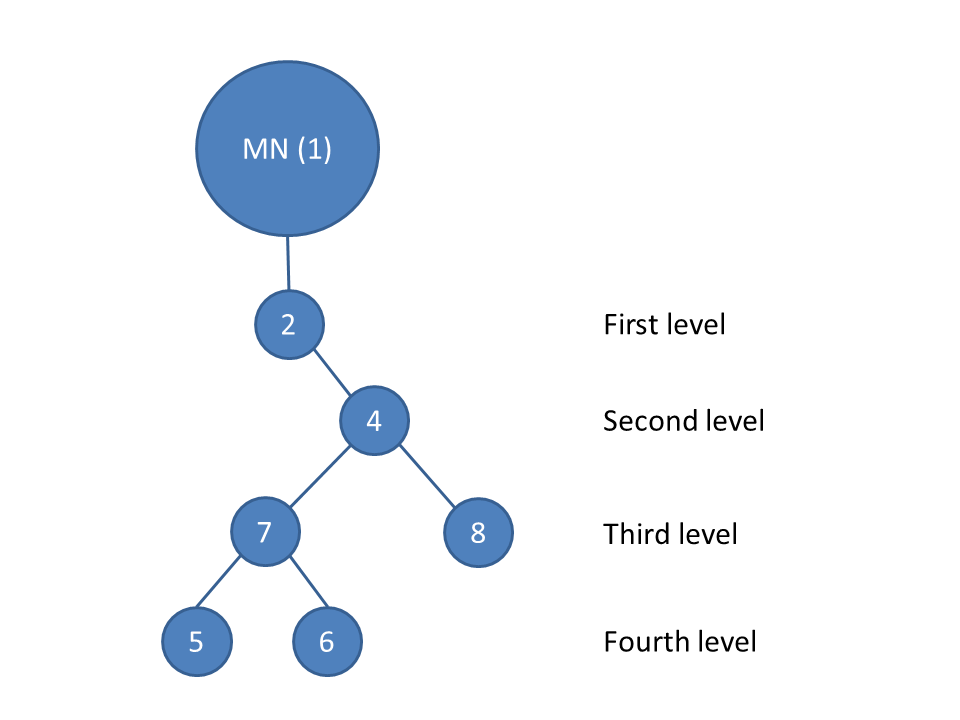
\includegraphics[width=0.8\textwidth]{chapters/design/figures/prottree2.png}}
	\caption{Example of a where node 3 disconnected.}
	\label{fig:prottree2}
\end{figure}

An example of this can be seen on Figure \ref{fig:prottree2}. This figure shows how node 3 disconnected, and now node 7 is attached to node 4 instead. This, of course, assumes that node 7 was in range of node 4.
This means that the next time data is requested, node 7 will be the parent for node 5 and 6, and they will now be a level higher than before.
